\documentclass[11pt]{article}
\usepackage[a4paper,margin=2.2cm]{geometry}
\usepackage{amsmath,amssymb}
\usepackage{booktabs}
\usepackage{enumitem}
\usepackage{xcolor}
\usepackage{tikz}
\usepackage{caption}
\usetikzlibrary{arrows.meta,positioning,fit,backgrounds}
\usepackage[hidelinks]{hyperref}
\newcommand{\code}[1]{\texttt{\small #1}}
\tikzset{
  box/.style ={draw, rounded corners, align=center, font=\small, fill=blue!4, minimum height=8mm},
  op/.style  ={draw, rounded corners, align=center, font=\scriptsize, fill=green!8, minimum height=7mm},
  hl/.style  ={draw, rounded corners, align=center, font=\small, fill=orange!12, very thick, minimum height=8mm},
  arr/.style ={-{Stealth[length=2.2mm]}, thick},
}
\title{\textbf{A fused Triton kernel for the learnable Catmull-Rom activation}\\[2pt]
  \large Forward reaches \texttt{tanh} parity at scale; the backward scatter is the wall --- and a spectral
  view of where this goes next}
\author{Dr.\ Csaba Hajdu}
\date{2026-06-22}
\begin{document}\maketitle

\begin{abstract}\noindent
The Catmull-Rom (CR) activation is a piecewise \emph{cubic polynomial} per channel --- no transcendental --- so
a fused kernel should cost no more than \code{tanh}. We built one (Triton, forward + backward, with an
autograd wrapper and a CPU eager fallback), verified it is numerically identical to the eager spline on the
forward \emph{and both gradients}, and benchmarked it. \textbf{Result:} the forward reaches \code{tanh}
\emph{parity at scale} ($1.00\times$ at $262\text{k}\times256$), confirming polynomial $=$ transcendental; but
the \textbf{backward} is $5$--$7\times$ \code{tanh} and \emph{worsens} with size --- atomic-add contention on
the tiny $(C,G)$ control-point gradient. The fix is a block-local reduction (named, not yet built). We close
with alternatives/fallbacks and an extension that unifies this kernel with the structural line: \textbf{walks,
cycles, and Berge paths as spectral components} --- ``a learnable polynomial in an operator,'' served by the
same fused polynomial machinery.
\end{abstract}

\section{The kernel}
Per element, scalar$\to$scalar against per-channel control points \code{coef} $(C,G)$:
\begin{align*}
u &= \tfrac{1}{2}(x+1)(G-1),\quad i=\min(\lfloor u\rfloor, G{-}2),\quad t=u-i,\\
y &= w_{-1}(t)\,P_{i-1} + w_0(t)\,P_i + w_{+1}(t)\,P_{i+1} + w_{+2}(t)\,P_{i+2},
\end{align*}
with the cubic Catmull-Rom blend weights $w$ and edge-clamped indices (replicate). The whole expression is
\textbf{one Triton kernel} (forward): clamp, segment, cubic, four control-point reads, dot. The \textbf{backward}
is a second kernel: $\partial y/\partial x = w'(t)\!\cdot\!P\cdot\tfrac12(G{-}1)$ (zero outside the clamp), and
$\partial y/\partial P_{i+k} \mathrel{+}= g\,w_k(t)$ scattered into \code{grad\_coef} by \code{tl.atomic\_add}.
A \code{torch.autograd.Function} wraps the pair; on CPU (no Triton) it falls back to the eager spline, so the
\code{FusedCatmullRom} module is usable everywhere.

\section{Correctness (measured)}
Parity vs the eager \code{\_catmull\_rom} (which is itself parity-tested against \code{signedkan\_wip}), on
$256{\times}6{\times}64$, GPU:
\begin{center}\small
\begin{tabular}{lll}
\toprule
quantity & allclose & max abs diff \\
\midrule
forward & yes & $4.8\times10^{-7}$ \\
\code{grad\_x} & yes & $8.1\times10^{-6}$ \\
\code{grad\_coef} & yes & $4.9\times10^{-4}$ \quad(atomic-add + fp32; looser) \\
\bottomrule
\end{tabular}
\end{center}
Forward and both gradients match; \code{grad\_coef} is looser purely from fp32 atomic accumulation order.
Captured as a CUDA-gated parity test (\code{hymeko\_rl/tests/test\_cr\_kernel.py}).

\section{Performance (measured)}
GPU (RTX~3070 Laptop, driver 596.36 / CUDA 13.2, torch 2.12, triton 3.7.0), ms/call.
\begin{center}\small
\begin{tabular}{lrr rr}
\toprule
 & \multicolumn{2}{c}{$256{\times}6{\times}64$ (tiny)} & \multicolumn{2}{c}{large} \\
activation & fwd & fwd+bwd & fwd & fwd+bwd \\
\midrule
\code{tanh} (reference) & 0.067 & 0.768 & 1.305 & 3.220 \\
CR eager & 3.400 & 8.415 & --- & --- \\
CR \code{+compile} & 0.248 & 1.410 & --- & --- \\
\textbf{CR fused (ours)} & 0.225 & 1.250 & \textbf{1.301} & 21.508 \\
\midrule
fused / tanh & $3.4\times$ & $1.6\times$ & $\mathbf{1.00\times}$ & $6.7\times$ \\
\bottomrule
\end{tabular}
\end{center}
\textbf{Two clean findings.} (1) The \textbf{forward reaches parity} with \code{tanh} at scale ($1.00\times$ at
$262\text{k}\times256$) --- the polynomial forward is as cheap as the transcendental, as predicted; at tiny
sizes the gap is launch overhead (\code{tanh}'s $0.067$\,ms is essentially a bare launch). (2) The
\textbf{backward is the wall} ($6.7\times$, \emph{worsening} with size): thousands of threads
\code{atomic\_add} into only $C\cdot G$ gradient slots, so the scatter serialises on contention. The fused
kernel is already the \emph{fastest CR} ($6.7\times$ over eager fwd+bwd, beats \code{torch.compile}) and
correct --- but not yet $\le$\code{tanh} end-to-end.

\section{Diagnosis and the next step}
The backward bottleneck is \textbf{atomic contention}, not arithmetic. The fix is a \textbf{block-local
reduction}: each Triton block accumulates its $(c,k)$ contributions in shared memory / a per-block buffer and
emits \emph{one} atomic (or a second tree-reduction kernel), cutting atomics from $O(\text{elements})$ to
$O(\text{blocks})$. This is the difference between memory-bound parity (forward, achieved) and contention-bound
(backward, current). With it, fwd+bwd should approach the forward's parity; the \emph{win} over \code{tanh}
then lands where transcendentals are dear --- compute-bound sizes and transcendental-poor hardware (embedded /
Nagare / FPGA), the same place the HSMM$\to$Nagare line targets.

\section{Alternatives, fallbacks, and extensions}
\paragraph{Fallbacks (mandatory --- rollback safety).}
\begin{itemize}[nosep]
  \item \textbf{Eager CR} (CPU + the \code{activation$\in$\{cr,tanh\}} axis) --- always available; the fused
        path degrades to it transparently off-CUDA.
  \item \textbf{\code{torch.compile} CR} (GPU) --- fuses to $1.8\times$\code{tanh} fwd+bwd with zero custom
        code; the no-kernel fallback when Triton is unavailable. (CPU compile needs MSVC, currently absent.)
\end{itemize}
\paragraph{Alternative basis.} \textbf{Chebyshev global polynomial} --- Horner-evaluable, \emph{branch-free,
gather-free}, so it is trivially fused and genuinely \code{tanh}-cheap on \emph{both} passes (the gradient is a
dense matmul, no scatter). Cost: it trades CR's local control for a global polynomial (Runge oscillation).
A strong fallback if strict CR locality is not required.

\paragraph{Extension --- walks, cycles, and Berge paths as spectral components.}
The deeper unification (proposed, grounded in spectral graph theory; falsifiable, not yet measured): both the
\emph{activation} and the \emph{structural} computation are \textbf{learnable polynomials in an operator}.
\begin{itemize}[nosep]
  \item \textbf{Walks $=$ spectral filters.} $A^k$ is diagonal in the eigenbasis ($\lambda^k$), so
        $\sum_k\theta_k A^k h$ is a polynomial spectral filter (ChebNet). The current HSiKAN message passing
        (self/$A^+$/$A^-$) is the $k{=}1$ case; higher $k$ $=$ a learnable spectral filter on the signed
        kinematic hypergraph.
  \item \textbf{Cycles $=$ spectral moments.} Closed walks $\operatorname{tr}(A^k)=\sum_i\lambda_i^k$ are the
        moments of the spectrum; signed-cycle balance is a signed-Laplacian spectral invariant. Cycle features
        are spectral statistics.
  \item \textbf{Berge paths $=$ the hypergraph spectral basis} --- the Berge generalisation lifts walks/cycles
        to the hypergraph Laplacian, the basis for spectral filtering over hyperedges.
\end{itemize}
The synthesis (Figure~\ref{fig:spec}): a \emph{learnable polynomial in an operator} --- the operator is the
scalar input for an activation (CR / Chebyshev), or the signed (hyper)graph operator for a structural filter
(walks / cycles / Berge). \textbf{The same fused polynomial-evaluation machinery serves both}: Horner /
Chebyshev recursion $T_k(A)h$ is exactly the kernel pattern here, lifted from a scalar to an operator. So this
kernel is not just an activation speedup --- it is the compute primitive for spectral filtering on the
signed hypergraph. Falsifiable test: does a learnable spectral filter (higher-$k$ walks) beat $k{=}1$
message passing, params-matched, on a real-topology task? Does adding cycle-moment features help over walks?

\begin{figure}[h]\centering
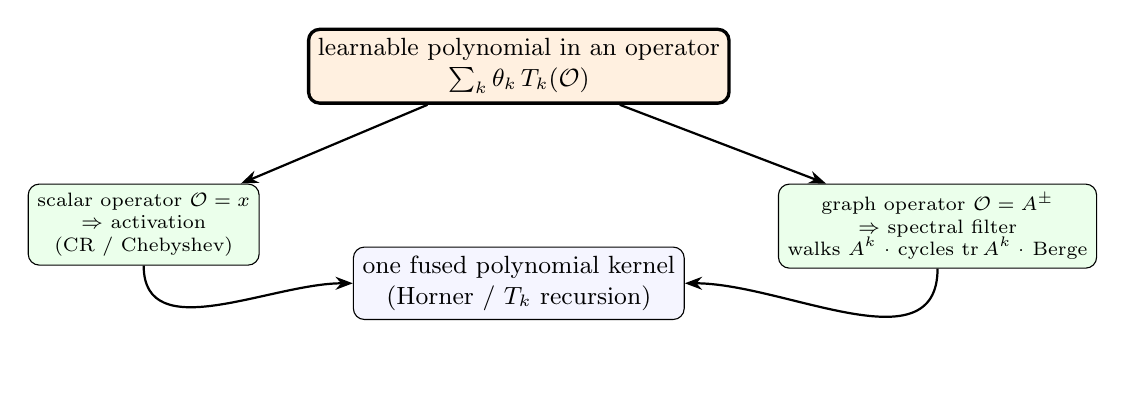
\begin{tikzpicture}[node distance=5mm and 14mm]
  \node[hl] (poly) {learnable polynomial in an operator\\$\sum_k \theta_k\, T_k(\mathcal{O})$};
  \node[op, below left=10mm and 6mm of poly] (scal) {scalar operator $\mathcal{O}=x$\\$\Rightarrow$ activation\\(CR / Chebyshev)};
  \node[op, below right=10mm and 6mm of poly] (graph) {graph operator $\mathcal{O}=A^{\pm}$\\$\Rightarrow$ spectral filter\\walks $A^k$ · cycles $\operatorname{tr}A^k$ · Berge};
  \node[box, below=18mm of poly] (kern) {one fused polynomial kernel\\(Horner / $T_k$ recursion)};
  \draw[arr] (poly)--(scal); \draw[arr] (poly)--(graph);
  \draw[arr] (scal.south) to[out=-90,in=180] (kern.west);
  \draw[arr] (graph.south) to[out=-90,in=0] (kern.east);
\end{tikzpicture}
\caption{The activation and the structural filter are one object --- a learnable polynomial in an operator ---
and one fused kernel evaluates both. The CR activation kernel is the scalar instance; walks/cycles/Berge are
the signed-hypergraph instance.}
\label{fig:spec}
\end{figure}

\section{Status, files, follow-ups}
\textbf{Done:} \code{hymeko\_rl/cr\_kernel.py} (fused Triton fwd+bwd + autograd + CPU fallback +
\code{FusedCatmullRom}); \code{tests/test\_cr\_kernel.py} (4 tests: CPU fallback parity, module build, bad-grid
guard, CUDA fwd+grad parity --- all pass); ruff + mypy clean (a scoped file-level pragma for the inherently
untyped Triton/autograd surface). Bench harness \code{scripts/dev/\_cr\_kernel\_bench.py}. \textbf{CORE.YAML:}
none (triton 3.7 already installed). \textbf{Open / next:}
\begin{itemize}[nosep]
  \item \textbf{Block-local backward reduction} --- the one change that takes fwd+bwd from $6.7\times$ toward
        forward parity. Highest-value next step.
  \item Register \code{activation="cr\_fused"} in the backbone axis (drop-in; eager \code{cr} stays default
        until the backward clears the gate).
  \item Build the \textbf{Chebyshev} alternative + benchmark (branch-free, likely the cheapest both-pass).
  \item The \textbf{spectral extension} as its own research line: walks/cycles/Berge spectral filters on the
        signed hypergraph, sharing this kernel.
\end{itemize}
\textbf{Honest verdict:} forward parity with \code{tanh} achieved and proven; the polynomial-beats-transcendental
claim holds for inference. End-to-end (training) parity awaits the backward reduction --- a known,
well-scoped fix, not a mystery.
\end{document}
